\documentclass{article}
\usepackage[utf8]{inputenc}
\usepackage{amsmath, amssymb, amsfonts}
\usepackage{tikz}
\usepackage{pgfplots}
\usepackage{cancel}
\usepackage[margin=3cm]{geometry}
%\usepackage{enumitem} % Allow tight lists
\usepackage{gensymb} % for degree symbol
\usepackage{tikzscale}

%\title{Robust control system development for VTOL-to-fixed wing flight %transition with the EcoSoar UAV}
%\author{Robert Hedman}
%\date{April 2019}


\begin{document}

\begin{titlepage}
    \begin{center}
        %\vspace*{1cm}
 
        \huge
        \textbf{Robust control system development for VTOL-to-fixed wing flight transition with the EcoSoar UAV}
 
        \vspace{0.5cm}
        \LARGE
        A thesis in Automatic Control
 
        \vspace{1.5cm}
 
        \textbf{Robert Hedman\\}
        \today
        \vspace{0.6cm}

        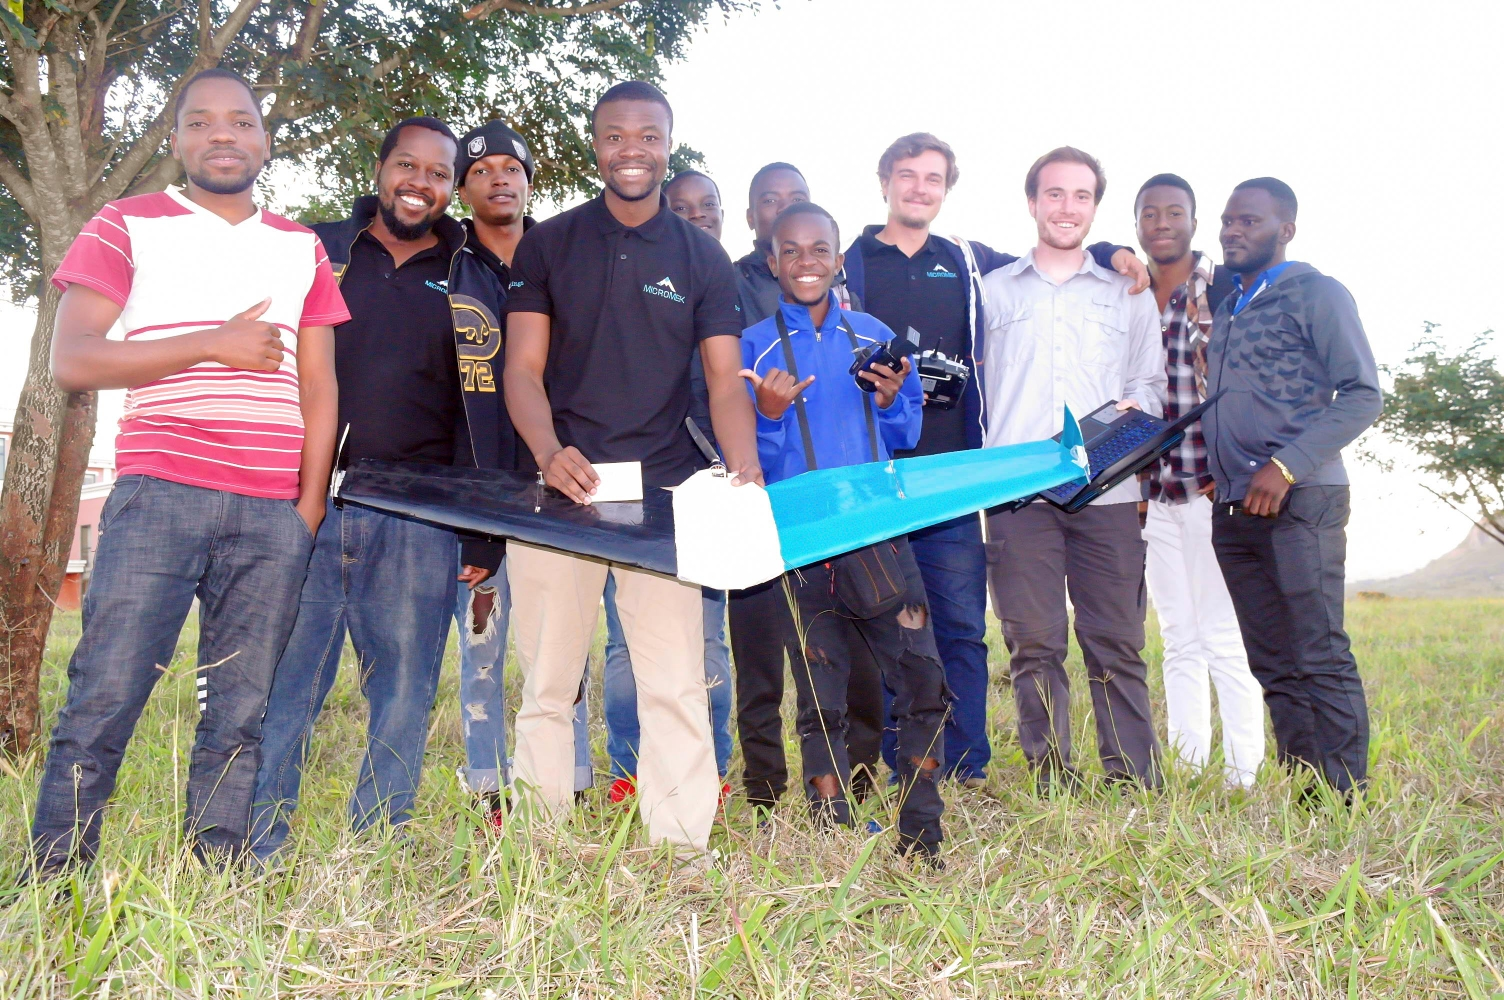
\includegraphics[width=0.9\textwidth]{coverphoto.jpeg}
 
        \vfill
 
        A thesis presented for the degree of\\
        Masters of Science / Civil Engineer
 
        \vspace{0.6cm}
 
        \Large
        Department of Computer Science, Electrical and Space Engineering\\
        Luleå University of Technology\\
        \textit{Supervisors:} K. \textsc{Atta}, K. \textsc{Kochersberger}\\
        \textit{Examinator:} G. \textsc{Nikolakopoulos}
 
    \end{center}
\end{titlepage}

\abstract
This is wehere we write about the abstract.
asdasdasd
asd
asdasdjhsdkjhdsak dikd  sdoj asodj asdoja sdojas do

\newpage
\section*{\textit{Acknowledgements}}

Thank Khalid, George, Mr. K, Avory, Wife, etc.

[Lets see if they require rent before adding below]\\
I also want to extend a very warm thank you to Montford Special Needs College in Malawi for allowing me to stay there together with my wife during this thesis.
The staff also provided all the support needed to become integrated with the local culture and helping out with practical issues such as getting a car, finding the hospital and providing a safe circle of friends.

\newpage

\tableofcontents

\newpage
\section{List of Variables}
%\begin{itemize}[topsep=0pt,itemsep=-1ex,partopsep=1ex,parsep=1ex]
\begin{center}\begin{tabular}{| c | c |} 
    $L_L$       & Lift from left wing \\
    $L_R$       & Lift from right wing \\
    $D_L$       & Drag from left wing \\
    $D_R$       & Drag from right wing \\
    $F_L$       & Lift due to aileron deflection, left side, outside propeller wake \\
    $F_{L_T}$   & Lift due to aileron deflection, left side, inside propeller wake \\
    $F_R$       & Lift due to aileron deflection, right side, outside propeller wake \\
    $F_{R_T}$   & Lift due to aileron deflection, right side, inside propeller wake \\
    $D_{\alpha_L}$ & Drag due to aileron deflection, left side, outside propeller wake \\
    $D_{\alpha_{L,T}}$ & Drag due to aileron deflection, left side, inside propeller wake \\
    $D_{\alpha_{R}}$ & Drag due to aileron deflection, right side, outside propeller wake \\
    $D_{\alpha_{R,T}}$ & Drag due to aileron deflection, right side, inside propeller wake \\
    $L_{W_L}$ & Lift from left winglet \\
    $L_{W_R}$ & Lift from right winglet \\
    $D_{W_L}$ & Drag from left winglet \\
    $D_{W_R}$ & Drag from right winglet \\
    $S_a$  & Surface area of one aileron, parts outside propeller wake \\
    $S_{a_w}$ & Surface area of one aileron, area inside propeller wake \\
    c.g.    & center of gravity (point) \\
    $T_L$   & Thrust from left propeller \\ 
    $T_R$   & Thrust from right propeller \\
    $S_w$   & Area of one wing, area outside of propeller wake \\
    $S_{w_w}$ & Area of one wing, area inside propeller wake \\
    $S_W$   & Area of one winglet \\
    $x_f$   & distance in $x$ from c.g. to aileron force \\
    $x_T$   & distance in $x$ from c.g. to thrust force \\
    $x_{ac}$& distance in $x$ from c.g. to wing aerodynamic center \\
    $x_W$   & distance in $x$ from c.g. to winglet force \\
    $y_T$   & distance in $y$ from c.g. to thrust force \\
    $y_f$   & distance in $y$ from c.g. to aileron force \\
    $y_{ac}$& distance in $y$ from c.g. to wing aerodynamic center \\
    $y_w$   & width of propeller wake \\ 
    $b$     & wingspan \\
    $z_W$   & distance in $z$ from c.g. to winglet force
\end{tabular} \end{center}
\newpage

\section{Background}
Virginia Tech, a University in Virginia, USA, has developed a fixed wing drone called the EcoSoar; a flying wing.
It is an aircraft designed for fabrication, operation and maintenance in low-
resource environments.
The total cost of one EcoSoar is only around 350 USD when costs for all tools and materials have been accounted for and spread over ten aircraft.

EcoSoar has been successfully flown in Malawi at
the test corridor established by UNICEF in Kasungu,
where a simulated payload of dried blood spot sam-
ples (used for HIV testing) was delivered 19 km from
a remote health clinic to the Kasungu airport. The
aircraft is constructed of poster-board and 3D printed
parts, making it easy to source in Malawi and low-
cost to repair if damaged.

Many flight operations occurring in Africa are converging on hybrid aircraft designs where the aircraft functions as a quadcopter in takeoff and landing but is capable of higher speed flight in a fixed wing configuration.

EcoSoar can currently be launched with a big bungee-cord or with a custom built launcher. It thus needs a field to both take off and land in since it can only land on its belly similar to that of any normal aircraft.
Modifying the EcoSoar to have two engines, one on the front of each wing, instead of the current design of having one at the back, might allow it to hover, take off and land vertically eliminating the need for a launching system as well as the requirement of a big field for take-off and landing.

Adding VTOL capacity to this drone would greatly increase its range of possible missions and thus help humanitarian efforts centered around EcoSoar in Malawi.

To achieve VTOL not only is hardware modifications necessary but also a new control scheme is necessary.

\section{Problem Forumulation}
This thesis will attempt to solve the problem of mathematically modeling a flying fixed wing, develop a VTOL capable model based controller that can handle both hovering, transitioning into flying and flying, and finally implement the controller on the Pixhawk controller onboard the aircraft.
Altering the aerodynamics of the EcoSoar is out of the scope for this thesis as is embedding the controller into fully fledged flight control system for example QGroundControl.
The project takes place in Malawi with very limited supply of electronics, spare parts, electricity, tools and lab equipment.

%Typically included as a subsection of the Introduction.
%Often accompanied by delimitations - statments about what is out of scope of the project.

%Formulation is incorrectly spelled.

\section{Needed math}
To develop this controller some basic concepts are required.
\subsection{General State Space background}
Many systems can be written as a set of differential equation.

Physical systems may sometimes be mathematically modeled by state space representation, given that it can be written on the same form as equation \ref{eq:generalstatespace} .
\begin{equation}
    \dot{\bar{x}} = f(\bar{x}) + g(\bar{u},\bar{x})
    \label{eq:generalstatespace}
\end{equation}
The states, $\bar{x}$ are related by a set of first order differential equations and some input.

Systems can have one input and one state, called Single Input Single Output (SISO), or have either multiple input and outputs or both; Multiple Input Multiple Output (MIMO) systems.
A system with several states, i.e. $\bar{x}$ being a vector, and several inputs, i.e. $\bar{u}$ being a vector is thus represented by a set of functions $\bar{f}$ and $\bar{g}$.

Diff. Eqs, state feedback, observability, controllability.
Are obs and contr. applicable on non linear systems?
MIMO
\subsection{State estimation/observers?}
\subsection{Feedback Linearization}
\subsubsection{Mimo: Lie derivatives and brackets}
\subsubsection{Decoupling matrix}
\subsection{L1 parameter compensation/estimation}
\subsection{Reference Frames}
NED, World+body frame
\subsection{Accellerated reference frames}
\subsection{Quaternions}
Motivate through problems with Euler angles, RPY, etc
Rotation matrix
Cover basic quaternion math,
world/bodyframe conversions
\subsubsection{Madgwick filter}
\subsection{Equations of Motion, in body frame}


\subsection {Basic aerodynamics}
An object moving through a medium displaces mass in the medium it travels through,
A wing moving through the air will displace air particles.
If the total movement of the particles generate a net momentum a force will be generated on the object displacing them, in this case the wing.

The air will thus excert pressure on the wing and it is useful to consider the pressure distribution.
By integrating the pressure distribution over the entire surface of the wing one can find the center of pressure.\cite{aerodynamics}
If the center of pressure and center of gravity are not aligned a torque will also be generated.
The equivalent force and moment can be placed at the center of pressure to simplify calculations.
The aerodynamic force can be split into two parts, one in line with the incoming airflow and one perpendicular to it.
These are usually denoted Lift and Drag forces, see figure \ref{fig:liftdrag} for an illustration of the Lift and Drag forces on an airfoil.

\begin{figure}[h]
    \center
    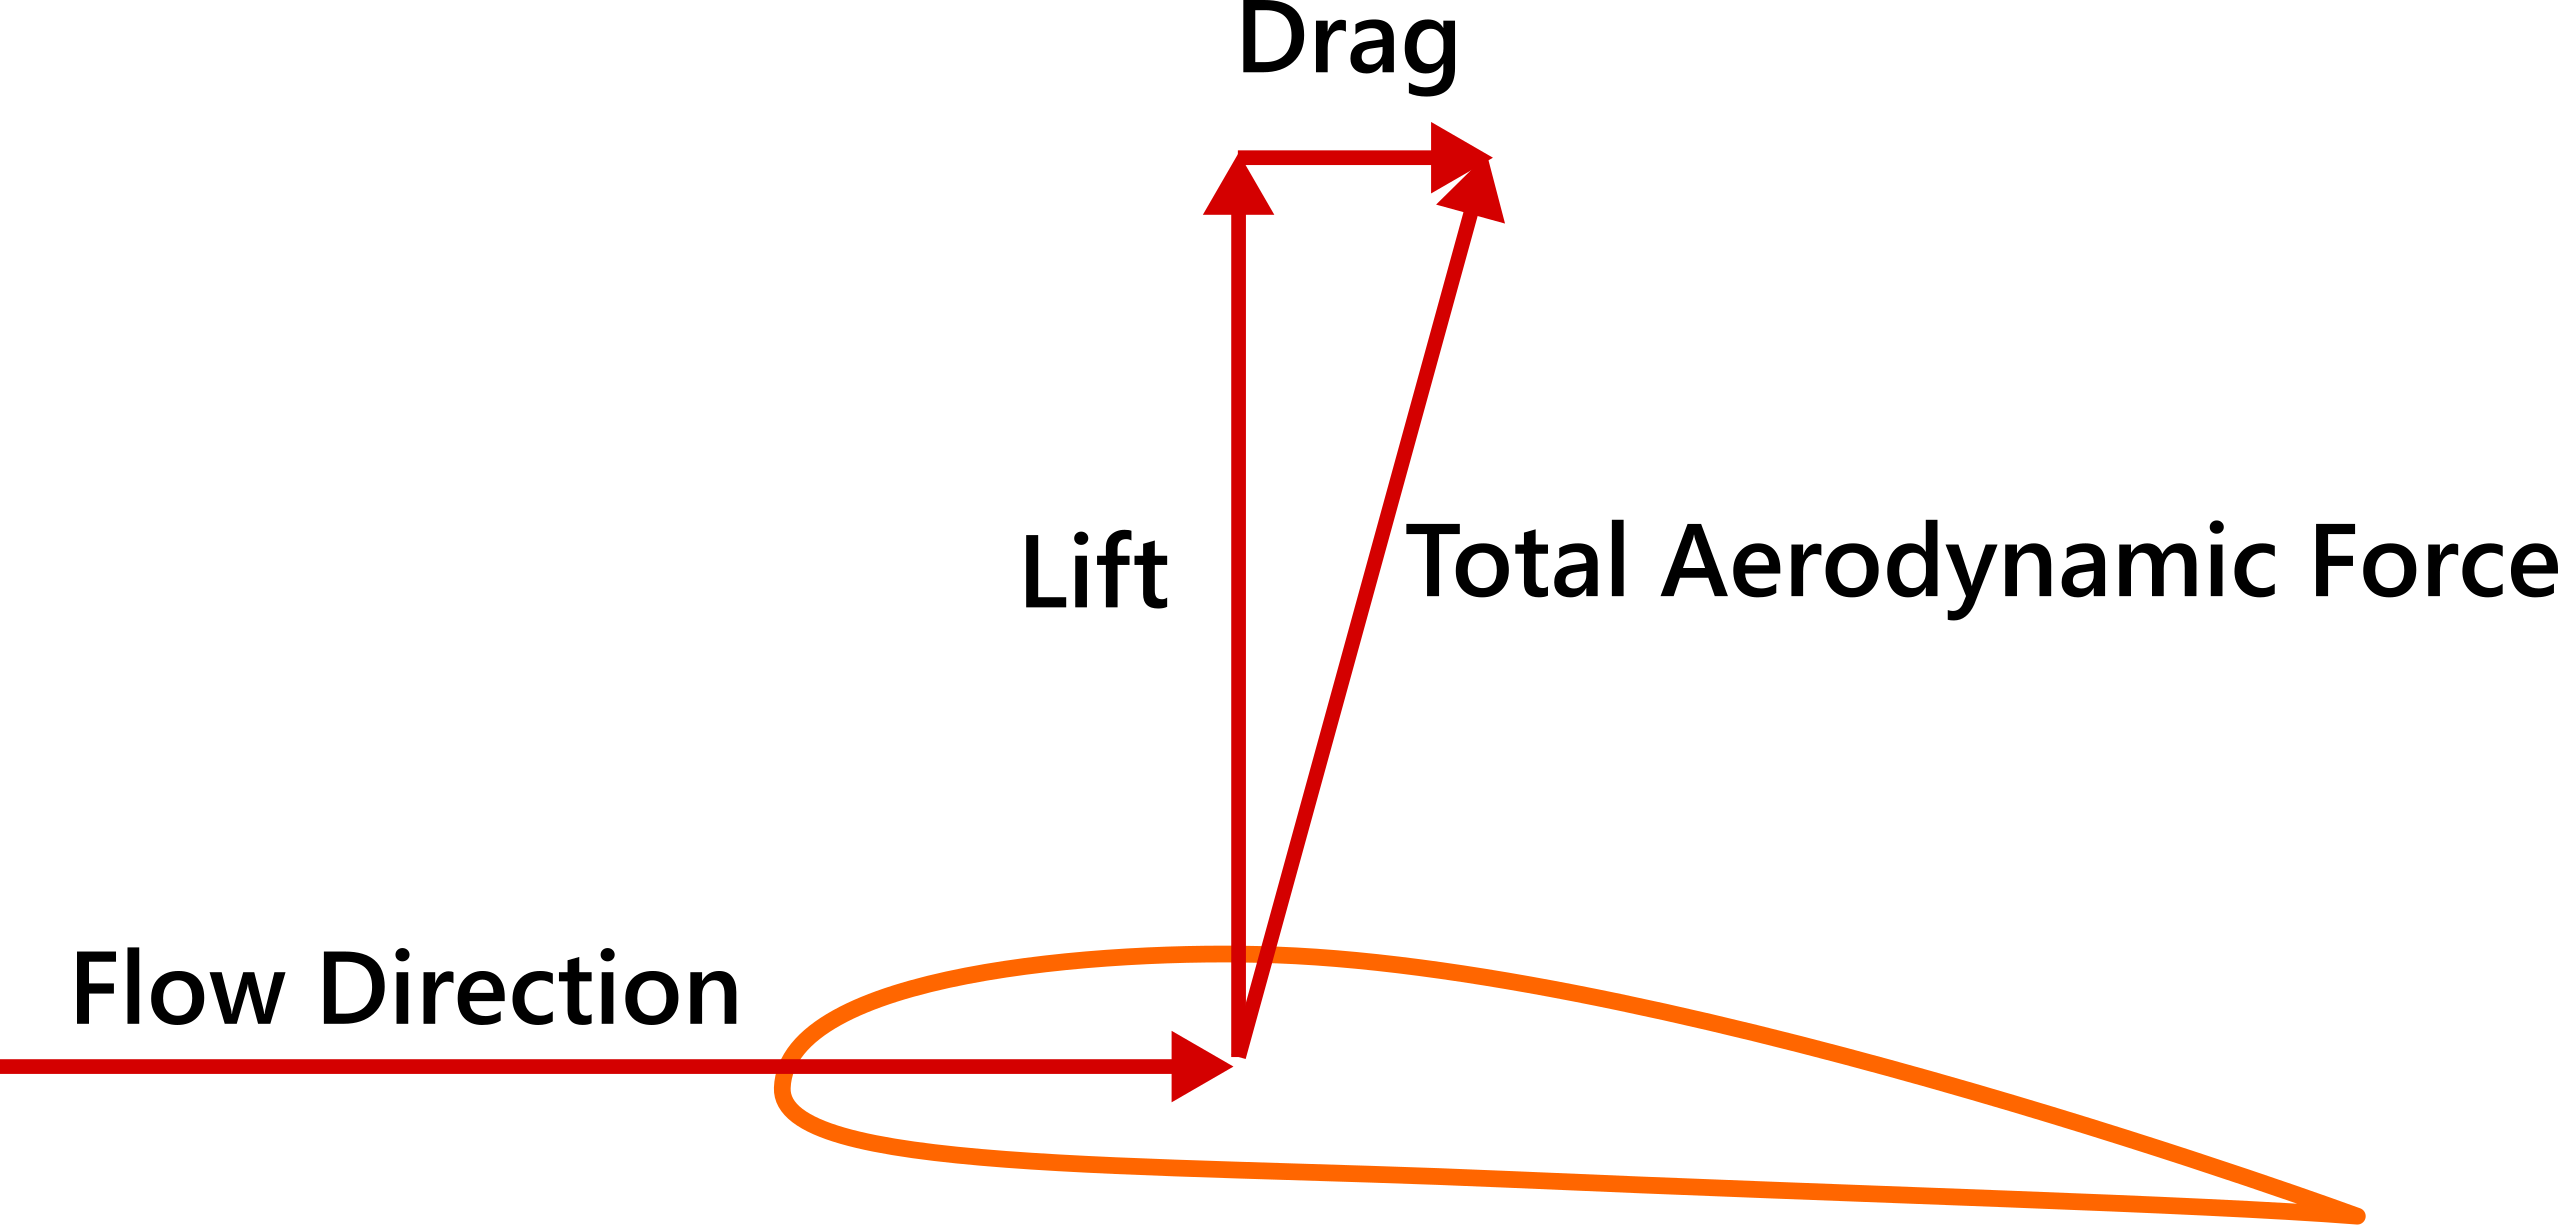
\includegraphics[width=0.4\textwidth]{liftdrag.png}
    \caption{An illustration of how the flow of air over an airfoil generate Lift and Drag. \cite{liftdragpng}}
    \label{fig:liftdrag}
\end{figure}

The lift force can further be broken down into several parts, but aerodynamics is a complicated field, and for the purposes of this thesis we only consider the following:
Lift due to camber (the non symmetry of the wing in the airstream), lift due to angle of attack (the angle which the incoming air makes with the wing) and lift due to control surface deflection.

\subsubsection{Propeller lift}
The force from propellers will be dealt with in greater detail further into this thesis.
But as an introduction they can be thought of as wings moving through the air, only in a rotational matter instead of straight on. 
As they move through the air lift is generated in a similair fashion to normal wings, but since the propeller is mounted at a right angle to the wings the lift force propels the aircraft forward.
The air a propeller displaces is called a wake and will be treated as a separate airflow from the aircraft moving through the air.


%\begin{itemize}
%        \item Bernoulli Equation, center of Pressure, etc
%        \item Basic plate theory
%        \item Aerodynamic center    
%        \item Aerodynamic forces and Moments
%        \begin{itemize}
%            \item Lift, and moment, due to camber
%            \item Lift due to angle of attack
%            \item Drag
%            \item Forces/Moments due to airflow over Ailerons and Elevators
%            \item Forces and Moments due to sideslip and roll
%            \item Forces/Moment due to roll rate, pitch rate and yaw rate
%        \end{itemize}
%        \item Propeller efficiency, airspeed, wake velocity
%    \end{itemize}
\begin{itemize}
        \item Bernoulli Equation, center of Pressure, etc
        \item Basic plate theory
        \item Aerodynamic center    
        \item Aerodynamic forces and Moments
        \begin{itemize}
            \item Lift, and moment, due to camber
            \item Lift due to angle of attack
            \item Drag
            \item Forces/Moments due to airflow over Ailerons and Elevators
            \item Forces and Moments due to sideslip and roll
            \item Forces/Moment due to roll rate, pitch rate and yaw rate
        \end{itemize}
        \item Propeller efficiency, airspeed, wake velocity
    \end{itemize}

\section{Mathematical Model of EcoSoar}


\section{Assumptions}

\begin{itemize}
    \item There is no external wind and so $v_{\infty}$ is replaced with $v$ which is the aircrafts velocity through the air.

    \item All forces operate on points in the $x-y$ plane, i.e. no offset in the $z$-direction (with the notable exception of the winglet forces). Forces may still have a $z$-component though.

    \item The propeller wake is unaffected by aircraft velocity, i.e. only determined by propeller speed.

    \item Airflow outside of wake is only determined by aircraft velocity.

    \item The aerodynamic centre (a.c.) is static and does not move with changes in speed and pressure. The moment around it, however, will vary and thus account for the effects of the a.c. movement.

    \item Airflow speed in wake is proportional to propeller rotational speed, $v_w = b_w \omega_i$, where $b_w$ is a constant.

    \item The principal moments axis align with the symmetry plane; only diagonal elements in the inertia matrix aligned with the body frame coordinate axis.

    \item Roll moment due to sideslip angle, negligible due to lack of tail with verical offset from c.g.

    \item Yawing moment due to roll rate is negligible due to the lack of a tail.

    \item Forces and moments due to acceleration are not explicitly calculated; they are already included in  dynamic model since it is based on forces.

\end{itemize}

\section{Coordinate system}
NED: North East Down.
$x$-axis is essentially the forward direction of the airplane in normal flying mode.
$z$-axis is pointed downwards.
$y$-axis is along the right wing.


\subsection{Aircraft force diagram}
The aircraft in question is the EcoSoar; a flying wing.
It has two control surfaces, one on each wing called elevons.
In front of each wing a motor and propeller is mounted providing thrust.
The motors also supply an airflow over the control surfaces when the aircraft is not moving through the air.


\begin{figure}[h]
    \center
    \begin{tikzpicture}
    \begin{tikzpicture}
    \begin{scope}[shift={(6,2.4)}]
    % Coord sys.
    \begin{scope}[shift={(1.2,-0.1)}]
        \draw[thick, ->] (-6,2) -- (-6,2.5) node[anchor=south east]{$x$};
        \draw[thick, ->] (-6,2) -- (-5.5,2) node[anchor=south west]{$y$};
        \draw[] (-6,2) circle (0.15cm);
        \draw[] (-6.1,1.9) -- (-5.9,2.1);
        \draw[] (-6.1, 2.1) -- (-5.9,1.9);
        \node[] at (-6.3,1.9) {$z$};
    \end{scope}

    % main body
    \draw (0,0) rectangle (1,2);
    % left wing
    \draw (0,2) -- (-5,0) -- (-5,-1) -- (0,0);
    % right wing
    \draw (1,2) -- (6,0) -- (6,-1) -- (1,0);
    % winglets, left and right
    \draw[very thick] (6,0) -- (6,-1);
    \draw[very thick] (-5,0) -- (-5,-1);

    % wingspan
    \draw[<->, thin] (-5,-2.2) -- (6, -2.2);
    \draw[dotted] (-5,-1) -- (-5, -2.5);
    \draw[dotted] (6, -1) -- (6, -2.5);
    \node at (0.5,-2.4) {$b$};

    % right Winglet forces
    \draw[fill=black] (6,-0.5) circle (0.05cm) ;
    \draw[->, thick] (6,-0.5) -- (6.5, -0.5);
    \node[] at (6.7,-0.8) {$L_{W_R}$};
    \draw[dotted] (6,-0.5) -- (7.2,-0.5);
    \draw[very thin, <->] (6.7,-0.5) -- (6.7, 1.4);
    \node[] at (7, 0.4) {$x_W$};

    \draw[->, thick] (6,-0.5) -- (6, -1.5);
    \node[] at (6.5,-1.5) {$D_{W_R}$};

    %left and right flaps
    %\draw (-4.4,-0.88) circle (0.1cm);
    %\draw (-1, -0.2) circle (0.1cm);
    \draw (-4.4, -0.88) -- (-4.4, -0.5) -- (-1, 0.25) -- (-1, -0.2);
    \draw (5.4, -0.88) --  (5.4, -0.5) -- (2, 0.25) -- (2,-0.2);

    % left and right propellers
    \draw[thick, ->] (-2.5,1) -- (-2.5,2) node[anchor=south east]{$T_L$};
    \draw[thick, ->] (3.5,1) -- (3.5, 2) node[anchor=south west]{$T_R$};

    % prop distance to cg
    \draw[<->] (-2.5, 2.5) -- (0.5, 2.5);
    \node[] at (-1, 2.7) {$y_T$};
    \draw[dotted] (3.5,2) -- (4.5,2);
    \draw[<->] (4.5,2) -- (4.5,1.4);
    \node[] at (4.8, 1.7) {$x_T$};

    % propeller cone. Left then Right
    \draw[dotted] (-3,2) -- (-3,-1);
    \draw[dotted] (-2,2) -- (-2,-1);
    \draw[dotted] (4,2) -- (4,-1);
    \draw[dotted] (3,2) -- (3,-1);

    % Propeller cone width
    \draw[<->] (4,-1) -- (3,-1);
    \node[] at (3.5, -1.2) {$y_w$};

    % Surface area aileron
    \node[] at (-2.5, -0.3) {$S_{a_w}$};
    \node[] at (-3.6, -0.53) {$S_a$};
    \node[] at (-1.6, -0.1) {$S_a$};

    % Wind surface areas
    \node[] at (2,0.8) {$S_w$};
    \node[] at (5,0) {$S_w$};
    \node[] at (3.35,0.85) {$S_{w_w}$};

    % Lift force, left
    \draw (-2.2, 0.4) circle (0.2cm);
    \draw[fill=black] (-2.2, 0.4) circle (0.025cm);
    \node[] at (-1.7, 0.4) {$L_L$};

    % Lift force, right
    \draw (3.2, 0.4) circle (0.2cm);
    \draw[fill=black] (3.2, 0.4) circle (0.025cm);
    \draw[dotted] (3.2, 0.4) -- (6.5,0.4);
    \node[] at (2.7, 0.4) {$L_R$};

    % Drag force, right
    \draw[->] (3.2,0.4) -- (3.2, -0.3);
    \node[] at (3.5,-0.3) {$D_R$};

    % Lift force distance
    \draw[<->] (0.5, -0.7) -- (3.2, -0.7);
    \node[] at (2, -0.5) {$y_{ac}$};
    % Right x distance
    \draw[<->] (6.2,1.4) -- (6.2, 0.4);
    \node[] at (5.8, 0.9) {$x_{ac}$};

    % Aileron force
    \draw (-2.5, -0.9) circle (0.2cm);
    \draw[] (-2.35, -0.75) -- (-2.65,-1.05);
    \draw[] (-2.65, -0.75) -- (-2.35, -1.05);
    %\node[] at (-2.4, -1.3) {$F_L$, $F_{L_T}$};
    \node[] at (-1.5, -1.0) {$F_L$, $F_{L_T}$};
    \draw[dotted] (-2.5, -0.9) -- (-5.5, -0.9);
    % Aileron drag
    \draw[->, thick] (-2.5, -0.9) -- (-2.5, -1.5);
    \node[] at (-1.4, -1.4) {$D_{a_L}$, $D_{a_{L,T}}$};

    % Distance flap force
    \draw[<->] (0.5,-1.8) -- (-2.5, -1.8);
    \node[] at (-1, -2) {$y_f$};
    \draw[<->] (-5.3, 1.4) -- (-5.3, -0.9);
    \node[] at (-5.6, 0.2) {$x_f$};

    % Center of Grav.
    \draw[fill=black] (0.5, 1.4) circle (0.1cm);
    \draw[dotted] (0.5,1.4) -- (0.5,-2);
    \draw[dotted] (0.5,1.4) -- (7.1,1.4);
    \draw[dotted] (0.5,1.4) -- (-5.5,1.4);
    \node[] at (0.55, 1.1) {c.g.};


    %mark 0,0
    %\draw (0,0) circle (0.1cm);

\end{scope}
\end{tikzpicture}
    \end{tikzpicture}
    \caption{Drawing of the EcoSoar, its propellers with wake and its control surfaces in body frame.}
    \label{airplane}
\end{figure}

The elevon forces, $F_L$, $F_{L_T}$, $D_{a_{L}}$ and $D_{a_{L,T}}$, have only been marked on the left wing, but exist symmetrically on the right wing with index $R$ instead of $L$.
The same is true for the drag force, $D_R$ and the winglet forces, $L_{W_R}$ and $D_{W_R}$, existing symmetrically on the left side.
$F_L$ is the force due to elevon deflection over surface area $S_a$, and $F_{L_T}$ is the force due to elevon deflection over $S_{a_w}$; the surface in the wake of the propeller.
Similarly for the drag, $D_{\alpha_L}$, $D_{\alpha_{L,T}}$, forces.
We also split the wing area into two sections: $S_w$ for the wing area outside the wake, and $S_{w_w}$ for the wing area in the wake.
The thrust forces, $T_i$, are assumed to act at the arrow end of the vector due to the offset in $x$ created by the motor and drive shaft.
The lift forces, $L_L$ and $L_R$, are functions of airflow over wing outside of wake and in the wake, which in turn are functions of aircraft velocity, propeller speed, angle of attack, air density, wing shape, etc.



\subsubsection{Aerodynamic Lift force}

The lift force of a wing depends on several factors.
Mainly: geometrical shape, dynamic pressure and angle of attack.\cite{aerodynamics}
The bigger the wing the more lift.
The faster air flows the more lift.
The further away from hitting the wing straight on, usually more lift.

Important note: Lift is defined as the \textbf{Aerodynamic force component perpendicular to the incoming airflow.} This means that, for example, the lift force labeled in figure \ref {airplane} as \textbf{$L_L$ is not the aerodynamic lift but rather the lift force in body frame.} The same argument applies to the drag forces.

Aerodynamic lift is usually modeled as\cite{nelson}\cite{aerodynamics}:
\begin{equation}
    L = Q  C_L S
\end{equation}
where $S$ is a reference surface area of the wing and $Q$ is the dynamic pressure:
\begin{equation}
    Q = \frac{1}{2} \rho v^2
\end{equation}
$\rho$ is the density of air and $v$ the velocity of the air hitting the wing.
$C_L$ is the coefficient of lift, a function of the angle of attack.
This coefficient is not linear. Empirical studies\cite{aoa180}\cite{aoa180-2} have found functions similair to the one in figure \ref{clalpha}.
\begin{figure}[h]
    \center
    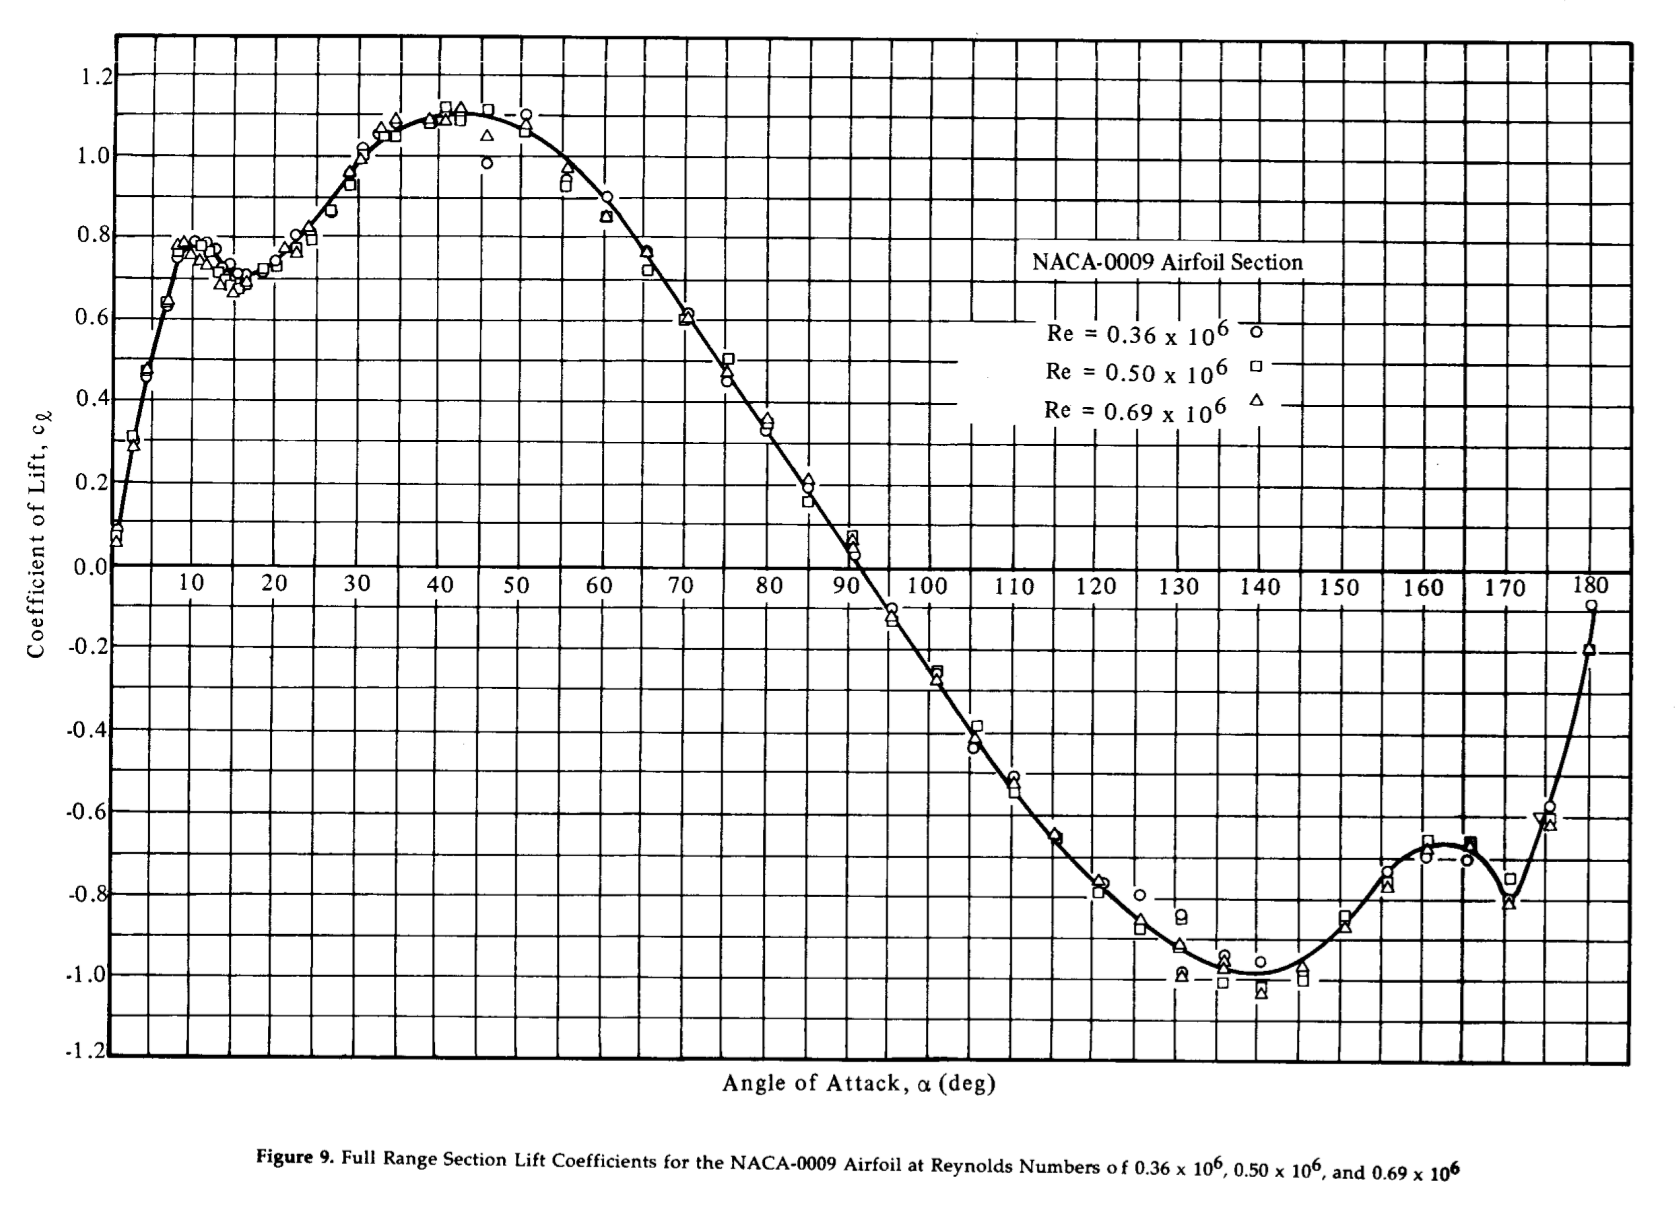
\includegraphics[scale=0.15]{aoa_80s.png}
    \caption{Coefficient of lift for a symmetrical wing vs angle of attack for the entire 180 degree rotation of the wing. The function is periodic.}
    \label{clalpha}
\end{figure}

The angle of attack, $\alpha$, is formally the angle at which the air is hitting the wing relative the body frame x-z axis.
If air is aligned with the $x$-axis $\alpha$ is zero, and if aligned with the $z$-axis $\alpha$ is 90.
(The airflow will obviously be in the negative axis direction since the airplane is flying in the positive direction and hitting the air).
Thus, if we assume no wind the angle of attack is only dependent on the aircraft velocity $\bar{v}$.
Normally this is modeled as:
\begin{equation}
    \alpha = tan^{-1}(\frac{v_z}{v_x})
    \label{eq:aoa}
\end{equation}
but in our case the velocity may have any direction in the $x$-$z$ plane, and is not limited to the right half plane.
The polar coordinates for vector $\bar{v}$ in the figure below, figure \ref{polar}, are:
\begin{equation}\begin{split}
    v_x =& \, r \, cos(\alpha) \\
    v_y =& \, r \, sin(\alpha) \\
    r =& \sqrt{v_x^2 + v_z^2}
    \label{eq:polar}
\end{split}\end{equation}
where $\alpha$ is in the interval $[-\pi,\pi]$.

\begin{figure}[h]
    \center
    \begin{tikzpicture}
    
    \draw[->] (-2,0) -- (2,0); % x-axis
    \node[] (x) at (2,-0.2) {$v_x$};
    \draw [->](0,-1) -- (0,2); % y-axis
    \node[] (y) at (0.3,2) {$v_z$};

    % Vector
    \draw[->, thick] (0:0) -- (90+45:1.5);
    \node[] at (90+45:1.7) {$\bar{v}$};

    % help lines
    \draw[dotted] (-1.05,0) -- (90+45:1.5);
    \draw[dotted] (0,1.05) -- (90+45:1.5);

    % angle
    \draw[->] (0.3,0) arc(0:45+90:0.3);
    \node[] at (0.3,0.4) {$\alpha$};
\end{tikzpicture}
    \caption{Velocity vector $\bar{v}$ in polar coordinates.}
    \label{polar}
\end{figure}

\subsubsection{Aerodynamic drag}
Similarly to aerodynamic lift the wing will also have an aerodynamic drag force, but parallel to the incoming flow and not perpendicular as lift.
The drag is also modeled like so:
\begin{equation}
    D = Q C_D S
\end{equation}
where the coefficient of drag, $C_D$, can also be experimentally obtained as in figure \ref{drag}.

\begin{figure}[h]
    \center
    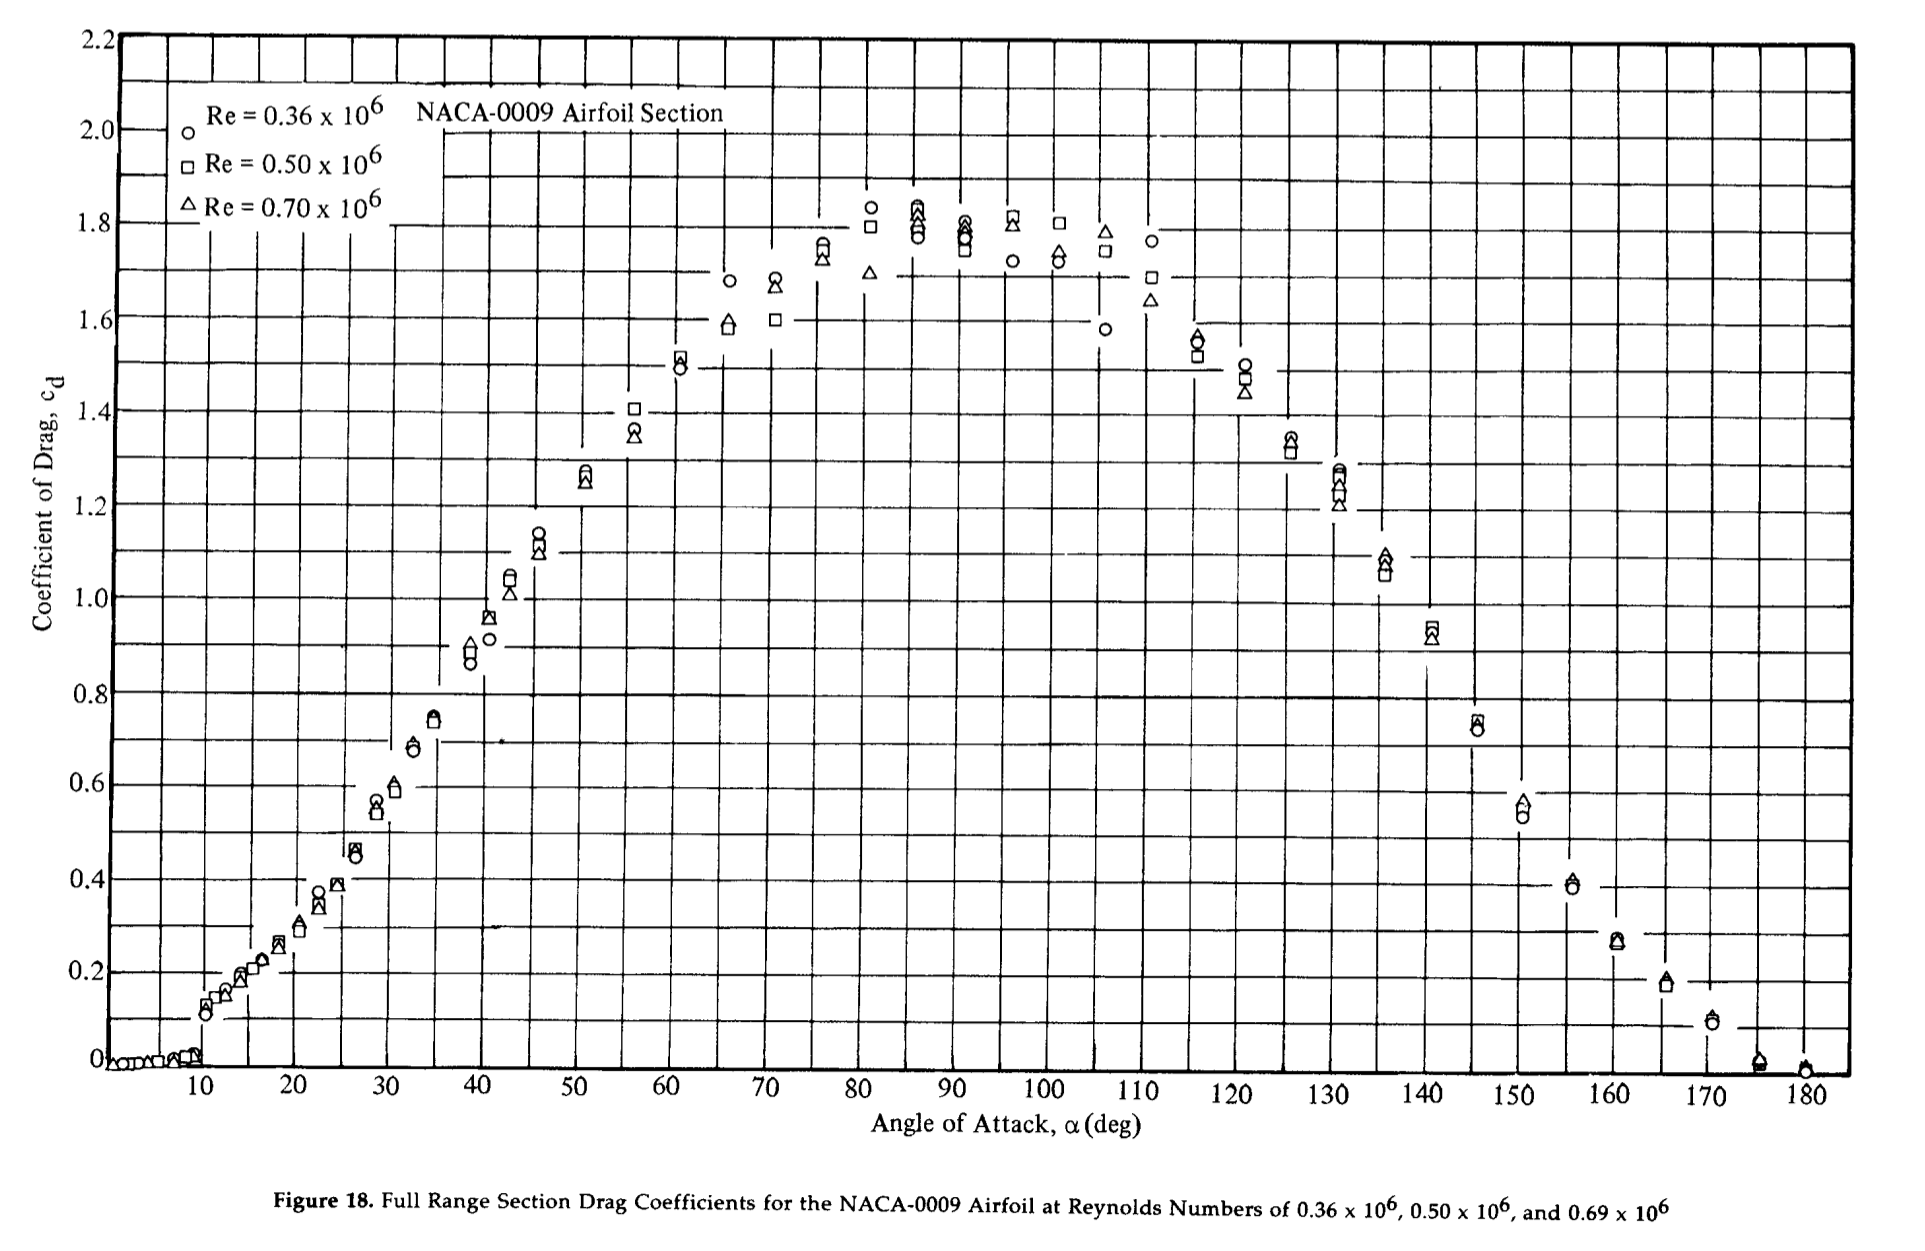
\includegraphics[scale=0.15]{drag180.png}
    \caption{Coefficient of drag for a symmetrical wing vs angle of attack for the entire 180 degree rotation of the wing.}
    \label{drag}
\end{figure}


\subsubsection{Lift and drag in body frame}

Since the aerodynamic lift and drag forces are relative the incoming airflow, i.e. functions of the angle of attack, $\alpha$, the body frame Lift and Drag have to transformed:
\begin{equation}\begin{split}
    L_i &= cos(\alpha) L + sin(\alpha) D \\
    D_i &= -sin(\alpha) L + cos(\alpha) D
    \label{LDbodyframe}
\end{split}\end{equation}
Note that the above forces are in the direction labeled in figure \ref{airplane} and not necessarily in the positive axis they act in.
From equation \ref{eq:polar} we see that
\begin{equation}\begin{split}
    v_x =& \, r \, cos(\alpha) \Rightarrow cos(\alpha) = \frac{v_x}{\sqrt{v_x^2 + v_z^2}} \\
    v_z =& \, r \, sin(\alpha) \Rightarrow sin(\alpha) = \frac{v_z}{\sqrt{v_x^2 + v_z^2}}
\end{split}\end{equation}
If we substitute in expressions for aerodynamic lift and drag we obtain:
\begin{equation}\begin{split}
    L_i =&  \frac{v_x}{\sqrt{v_x^2 + v_z^2}} Q C_L S +
            \frac{v_z}{\sqrt{v_x^2 + v_z^2}} Q C_D S \\
    D_i =& -\frac{v_z}{\sqrt{v_x^2 + v_z^2}} Q C_L S +
            \frac{v_x}{\sqrt{v_x^2 + v_z^2}} Q C_D S \\          
\end{split}\end{equation}
which simplify into:
\begin{equation}\begin{split}
    L_i =& 
     S \frac{1}{2} \rho v^2 \left( \frac{C_L v_x + C_D v_z}{\sqrt{v_x^2 + v_z^2}} \right) \\
     %
    D_i =& 
     S \frac{1}{2} \rho v^2 \left( \frac{-C_L v_z + C_D v_x}{\sqrt{v_x^2 + v_z^2}} \right)
     \label{liftdragbody}
\end{split}\end{equation}
where $v = \sqrt{v_x^2 + v_y^2 + v_z^2}$.


\subsection{Moment due to force}

Any force not acting at the center of gravity will produce a moment around c.g.
The moment of a force is:
\begin{equation}
    \bar{M} = \bar{r} \times \bar{F}
\end{equation}
With our assumptions the above equation can be written as:
\begin{equation}
    \bar{M} = (r_x, r_y, 0) \times (F_x, F_y, F_z) = 
    \left[ \begin{matrix}
    F_z r_y \\
    -F_z r_x \\
    F_y r_x - F_x r_y \end{matrix} \right]
\end{equation}

\subsubsection{Pitching moment}
Lift due to camber on a wing acts at ~50\% of the cord line.
Lift due to angle of attack acts at roughly 25\% of the cord line.\cite{aerodynamics}
This makes the force acting point, center of pressure, move along the cord line when angle of attack and aircraft velocity changes.
A common simplification is to choose the aerodynamic center, a.c., as the point at which Lift acts.
It can be shown that placing the a.c. at the 25\% cord position 
makes the moment generated vary little as angle of attack changes, yielding simpler equations.
The pitching moment due to lift can now be expressed as:
\begin{equation}
    \tau_{y,lift} = \sum_{j \in [w, w_w]}
    C_{m,y,l} Q S_j l +  \cancelto{0}{\sum_{j \in [w, w_w]}
    C_{m,y,l,\alpha} Q S_j l \alpha}
\end{equation}
where $l$ is the characteristic length of the wing, usually taken as the mean cord for pitching moments and the wingspan for rolling and yawing moments.

\subsection{Equations of motion}

The equations of motion can be split into three parts: one part due to gravity, one part due to the rigid body frame being an accelerated reference frame, and one part due to aerodynamic forces.
These forces depend on the aircrafts attitude and will be expressed in terms of it.

\subsubsection{Attitude}
The attitude is represented by a quaternion:
\begin{equation}
\bar{q} = [q_0, q_1, q_2, q_3]^T
\end{equation}
Any vector, $\bar{r}_w$, in world frame can be represented in the body frame by the conversion:
\begin{equation}
    \bar{r}_b = \bar{q} \bar{r}_w \bar{q^*}
\end{equation}

\subsubsection{Gravity}
In the case of gravity, $\left[\begin{smallmatrix}0\\0\\mg\end{smallmatrix}\right]_w$, the force, $m \bar{g}$, becomes
\begin{equation}
m \dot{\bar{v}}_b = \left[ \begin{matrix}
    2 (\bar{q_1} \bar{q_3} + \bar{q_0} \bar{q_2})  \\
    2 (\bar{q_2} \bar{q_3} - \bar{q_0} \bar{q_1})  \\
    (\bar{q_0}^2 - \bar{q_1}^2 - \bar{q_2}^2 + \bar{q_3}^2) 
    \end{matrix} \right] m g
\end{equation}
Gravity acts in the center of gravity and creates no moment.
Since gravity is in world frame and we want to express it in body frame we need to conjugate the quaternion.

\subsubsection{Forces and moments due to accelerated body reference frame}

In the case of a rigid body with inertia matrix $I$, velocity $\bar{v}$ and angular velocity $\bar{\omega}$ relative a fixed frame we have the moment equation:
\begin{equation}
    I \dot{\bar{\omega}} = \bar{\tau} - \bar{\omega} \times
    I \bar{\omega}
\end{equation}
where $\tau$ is the external torque acting on the body.

Similarly, if we include the coriolis force we obtain the forces in our body frame:
\begin{equation}
    \bar{F} = \bar{F}_{e} 
    + 2 m \, \bar{\omega} \times \bar{v}
\end{equation}
where $\bar{F_e}$ is the external forces acting on the body.
No other inertial forces are of interest;
the linear accelleration is irrelevant since we are not flying inside a linearly accellerating frame, and the other two depend on rotation around a non principal axis.

In our case, with assumptions made, the above equations simplify to:

\begin{equation}
\left[
\begin{matrix}
    \dot{\bar{v}} \\
    \dot{\bar{\omega}}
\end{matrix} \right]
=
\left[
\begin{matrix}
    \dot{v_x} \\
    \dot{v_y} \\
    \dot{v_z} \\
    \dot{\omega_x} \\ 
    \dot{\omega_y} \\
    \dot{\omega_z}
\end{matrix} \right] 
=
- \left[ \begin{matrix}
2 ( v_z \omega_y - v_y \omega_z )\\
2 ( v_x \omega_z - v_z \omega_x )\\
2 ( v_y \omega_x - v_x \omega_y )\\
\frac{1}{I_x} (I_z - I_y) \omega_y \omega_z \\
\frac{1}{I_y} (I_x - I_z) \omega_x \omega_z \\
\frac{1}{I_z} (I_y - I_x) \omega_x \omega_y 
\end{matrix} \right]
+ \verb!external forces and moments!
\end{equation}


\subsubsection{elevons}
Aileron forces are modeled similarly to lift, as well, but with an extra term, $\delta_i$, for the deflection degree in radians:
\begin{equation}
    F_i = C_{L_\delta} \sum_{j \in [a, a_w]}  Q_{j,i} S_j \delta_i
\end{equation}
and similairly the drag created by the ailerons:
\begin{equation}
    D_{\alpha_i} = C_{D_\delta} \sum_{j \in [a, a_w]}  Q_{j,i} S_j \delta_i
\end{equation}
The aileron lift, and drag, coefficient is assumed to be static over all angle of attacks since they will be in the wake of the wing, and the lift and drag are linear in the region of angles the ailerons can deflect.


\subsection{Winglets, forces and moments due to sideslip}
The aircraft considered here has no tail nor separate body (as the body is part of the wing).
The only surfaces providing relevant forces due to sideslip are the winglets.
The winglets each have an area $S_W$ and are flat plate wings which will generate aerodynamic lift and drag forces due to $\beta$ providing an angle of attack in their reference frame.
$\beta$ can be, similarly to $\alpha$, be expressed in polar coordinates:
\begin{equation}\begin{split}
    v_x =& \, r \, cos(\beta) \\
    v_y =& \, r \, sin(\beta) \\
    r =& \sqrt{v_x^2 + v_y^2}
\end{split}.
\end{equation}
Note that $\beta$ is in the $x$-$y$ plane and not $x$-$z$ plane as in the case for $\alpha$.
$\beta$ can be described as the horizontal incoming angle relative the airfraft body frame and since the winglets are vertical this will act as their angle of attack.


The aerodynamic forces, $L_\beta$ and $D_\beta$, from the winglets convert into body forces, as in figure \ref{airplane}, similarly to lift and drag from the main wings:
\begin{equation}\begin{split}
L_{W_i} &= cos(\beta) L_\beta +  sin(\beta)D_\beta \\
D_{W_i} & = -sin(\beta) L_\beta + cos(\beta) D_\beta
\end{split}\end{equation}
where
\begin{equation}\begin{split}
L_\beta &= Q C_{L_\beta} S_W \\
D_\beta & = Q C_{D_\beta} S_W
\end{split}\end{equation}
and $C_{k_\beta}$ are the lift and drag coefficients for each winglet, here assumed to be flat plates.
$v_z$ can be assumed to be negligible in the following equations since the physics from the main wings will dominate the effects due to $v_z$.
If we assume $v_z$ to be negligible then we obtain:
\begin{equation}\begin{split}
L_{W_i} &= 
    \frac{\rho v S_W}{2}  \left( C_{L_\beta} v_x + v_y C_{D_\beta} \right) \\
%
D_{W_i} &= 
    \frac{\rho v S_W}{2 }  \left(-v_y C_{L_\beta} + v_x C_{D_\beta} \right)
\end{split} .
\end{equation}
If the sideslip angle, $\beta$, is small (which implies $v_y$ small) the lift and drag coefficients can be approximated as 
\begin{equation}\begin{split}
    C_{L_\beta} \approx& \frac{d C_{L_\beta}}{d \beta} \big\vert_{\beta=0} \, \beta \\
    C_{D_\beta} \approx& 0
\end{split}\end{equation}
where the Lift coefficient is assumed linear with respect to $\beta$, which makes sense looking at figure \ref{clalpha}.
Similarly, Drag for a flat plate is roughly zero around zero angle of attack.
This results in:
\begin{equation}\begin{split}
L_{W_i} &\approx 
    \frac{\rho v S_W}{2} \frac{d C_{L_\beta}}{d \beta} \big\vert_{\beta=0} \, \beta \, v_x  \\
%
D_{W_i} &\approx 0
\end{split}\end{equation}
This gives us, in body frame, one restoring force from each winglet roughly proportional to the forward velocity squared of the aircraft and the sideslip angle..
The forces have the same magnitude and direction on both sides of the aircraft.



\subsubsection{Restoring moment}

$D_{W_i}$ are symmetrical on both sides and only create an acceleration in $y$.
They do not generate any moment.
$L_{W_i}$, however, act asymmetrically around c.g.~and do generate a torque (note that the force $L_{W_R}$ generates a negative torque around $z$ in our coordinate system):
\begin{equation}
    M_z = L_{W_L} x_W + L_{W_R} x_W = - \rho v S_W \frac{d C_{L_\beta}}{d \beta} \big\vert_{\beta=0} \, \beta \, v_x x_W
\end{equation}

\subsubsection{Non linear forces and moments}
If we do not make the assumption that $\beta$ is small we instead get the equations:
\begin{equation}\begin{split}
    M_z =& - \, x_W \rho v S_W  \left( C_{L_\beta}(\beta) v_x + v_y C_{D_\beta}(\beta) \right) \\
    D_{W} =& \rho v S_W \left(-v_y C_{L_\beta}(\beta) + v_x C_{D_\beta}(\beta) \right)
\end{split}\end{equation}
where $D_W = D_{W_L} + D_{W_R}$, and the coefficients of lift and drag are as shown in the figures \ref{clalpha} and \ref{drag}, but functions of $\beta$ instead of $\alpha$ as $\beta$ becomes the effective angle of attack in the winglets reference frame.



\subsubsection{Rolling moment due to sideslip}

The center of the winglet is slightly offset in the $z$-direction from the c.g. by distance $z_W$. 
Given the forces $L_{W_i}$ the rolling moment due to sideslip, $M_x$, is simply
\begin{equation}
    M_x = z_W (L_{W_L} + L_{W_R})
\end{equation}



\subsection{Propeller Thrust}
Thrust will be modeled as
\begin{equation}
    T_i = K_T \omega_i^2
\end{equation}
where $K_T$ is the thrust coefficient of the propeller and $\omega_i$ the rotational speed of the propeller.

Behind the propellers an area of airflow is generated, called a wake.
Given a propeller diameter of $d_P$, pushing air through at a rate of $v_w$ the volume of air being moved by the propeller during time $t$ is:
\begin{equation}
	V_{air} = \int_0^t \frac{d}{2} \pi^2 v_w dt \,.
\end{equation}
The air has density $\rho$ converting the volume into mass:
\begin{equation}
	m_{air} = \rho \, m_{air}
\end{equation}
If we assume the air to be stationary in front of the propeller and the aircraft standing still the change in momentum in the air is:
\begin{equation}
	\Delta p = m_{air} v_{air} = \rho \frac{d \pi^2}{2} v_w^2 t
\end{equation}
Force due to change in momentum is:
\begin{equation}
	F t = \Delta p \Rightarrow F = \frac{\Delta p}{t}
\end{equation}
giving us:
\begin{equation}
	F = \rho  \frac{d \pi^2}{2} v_w^2 \, .
\end{equation}
By combining all parameters into one coefficient $K_v$, the following equation is obtained:
\begin{equation}
	F = K_v  v_w^2 \, .
\end{equation}

If we instead look at the lift generated by the propeller blades we can find the thrust as a function of propeller rotation speed.
Assuming the aircraft has no speed and there is no wind we can model the lift from one propeller blade as:
\begin{equation}
	L_i = \int_0^{\frac{d}{2}} \frac{\rho}{2} (\omega_i r)^2 C_L(pitch) dr
\end{equation}
If we also assume a constant pitch along the diameter of the propeller blade the above integral simplifies into:
\begin{equation}
	L_i = \frac{\rho d^3}{48} C_L(pitch) \omega_i^2
\end{equation}
and thus with $n$ blades we find the total lift, i.e. thrust:
\begin{equation}
	T_i = L = \sum_{i \in [1,n]} L_i = n L_i
\end{equation}

By comparing the equation for thrust due to rotation speed and thrust due to airflow we conclude that:
\begin{equation} \begin{split}
	K_v v_w^2 =& n \frac{\rho d^3}{48} C_L(pitch) \omega_i^2 \Rightarrow \\
	& v_w = b_w \omega_i
\end{split}\end{equation}
and so the assumption that airflow in the wake is proportional to the propeller angular speed holds.



\subsection{Restoring moment due to roll rate}
If we assume that $v_y$ is negligible then the Lift and Drag forces in body fram simplify into:
\begin{equation}\begin{split}
    L_i =& 
     S \frac{1}{2} \rho v^2 \left( \frac{C_L v_x + C_D v_z}{\sqrt{v_x^2 + v_z^2}} \right) = 
      S \frac{1}{2} \rho \sqrt{v_x^2 + v_z^2} \left(C_L v_x + C_D v_z \right)\\
     %
    D_i =& 
     S \frac{1}{2} \rho v^2 \left( \frac{-C_L v_z + C_D v_x}{ \sqrt{v_x^2 + v_z^2}} \right)
     = S \frac{1}{2} \rho \sqrt{v_x^2 + v_z^2} \left(-C_L v_z + C_D v_x\right)
     \label{liftdragbody}
\end{split}\end{equation}
If the plane is experiencing rolling, a rotation about the $x$-axis with a rotational speed of $\omega_x$ then a restoring moment will be created.
This is because the air is resisting the wings motion through the air.

The rotational speed will yield an increased local $v_z$, $v_{z,l}$, along the wing:
\begin{equation}
    v_{z, l} = v_z + \omega_x y
\end{equation}
where $y$ is the distance away from the body along the wing.
The change in velocity changes the angle of attack locally.
The local angle of attack is denoted $\alpha_l$.

Lets consider the full moment as the integral of the full moment across both wings.
This way the symmetrical lift forces will cancel and only the rolling moment will remain.
\begin{equation}\begin{split}
    M_x =& -\int_{-b/2}^{b/2} y dL_i(y) dy \\
    =& -\frac{\rho}{2}\int_{-b/2}^{b/2} y c(y) \sqrt{v_x^2 + v_{z,l}^2} \left(C_L v_x + C_D v_{z,l} \right) dy \\
\end{split}\end{equation}
If we make the crude assumption that $C_L = a * sin(2*\alpha)$, and the less crude asumption that $C_D = -b * cos(\alpha) + b$, it is still impossible to find the function $M_x(\omega_x)$ for the entire state space.
A term:
\begin{equation}
    \int_{-b/2}^{b/2} y \sqrt{(v_1 + \omega y)^2 + v_2^2} dy
\end{equation}
will remain, and one has to assume $\alpha \in [-\pi/2, \pi/2]$, $v_2 \neq 0$ and/or many of the variables always positive, to find the function without the integral.

A simulator can solve the integral numerically but in order to find smooth analytical expressions for the controller approximations have to be made.

It turns out that the four dimensional function for restoring moment due to roll as a function of roll rate $\omega_x$, $v_x$ and $v_z$ is actually quite linear with respect to $\omega_x$.
The remaining function can be closely approximated by a two dimensional polynomial in $v_x$ and $v_z$ allowing for a feedback linearized model to be implemented with very little error.
This can also help with computational efficiency should an estimator need to run onboard the aircraft.

\subsection{Restoring moment due to yaw rate}
Similarly the restoring moment due to yaw rate can be obtained from the following integral:
\begin{equation}\begin{split}
    M_z = 
    % restmom yaw rate
    & \int_{-b/2}^{b/2} y \left( \frac{1}{2} \rho \sqrt{v_{x,l}^2 + v_z^2} \left( -C_L v_z + C_D v_{x,l} \right) \right) c(y) dy
\end{split}\end{equation}
where $v_{x,l} = v_x - \omega_z y$.

%For the controller some linear approximation has to be found, similarly as to restoring moment due to roll rate.

\subsection{Rolling moment due to yaw rate}
Due to the change in forward velocity a change in lift is also produced, inducing a rolling moment obtained similarily:

\begin{equation}
	M_x = \int_{-b/2}^{b/2} y \left( \frac{1}{2} \rho \sqrt{v_{x,l}^2 + v_z^2} \left( C_L v_{x,l} + C_D v_{z} \right) \right) c(y) dy
\end{equation}
where $v_{x,l} = v_x - \omega_z y$.

For the controller some linear approximation has to be found, similarly as to restoring moment due to roll rate.

\subsection{Restoring moment due to pitch rate}
Due to the absence of a tail this moment will be much smaller than on aircraft with a tail.
Most of the wing surface area is behind the center of gravity, and due to the wing sweep more surface will be at a longer distance from c.g. in $x$ direction.
This means that we can approximate the entire wing to be behind the c.g.
This aircraft also has a relatively small inertia around the $y$ axis; the aircraft will quickly turn into the wind.

Since we have modeled the lift in such a way that the pitching moment does not vary with angle of attack we can assume here that it is only proportional to the aircraft velocity and $\omega_y$.
Similarly as in section \ref{sec:restmomroll}, but with constants instead of coefficients of lift and drag, giving us the following expression directly:
\begin{equation}
    M_y = -\omega_y \rho S \sqrt{v_x^2 + v_z^2} C_{D,\omega_y} \frac{x_{\omega_y}^2}{24}
    =
    -\omega_y \rho S C_{\omega_y} \sqrt{v_x^2 + v_z^2}
\end{equation}
where $C_{\omega_y}$ is some constant that needs to be approximated experimentally.



\subsection{Actuator dynamics}
The actuators onboard are not direct term but contain some dynamics.
In this thesis they will be modelled as first order systems.
\subsubsection{elevon dynamics}
Given an input signal $u_{\delta_i}$ for elevon $i$ we model the deflection, $\delta_i$, like so:
\begin{equation}
    \dot{\delta_i} = K_{\delta_i} (-\delta_i + u_{\delta_i})
\end{equation}

\subsubsection{Motor dynamics}
Given an input signal $u_{\omega_i}$ we model the motor dynamics as so:
\begin{equation}
    \dot{\omega_i} =  K_{\omega_i}(-\omega_i + u_{\omega_i})
\end{equation}


\subsection{Full equations of motion}

We now include all terms to find the full state space equations:

\begin{equation}
\left[
\begin{matrix}
    \dot{v_x} \\
    \dot{v_y} \\
    \dot{v_z} \\
    \dot{\omega_x} \\ 
    \dot{\omega_y} \\
    \dot{\omega_z} \\
    \dot{q_0} \\
    \dot{q_1} \\
    \dot{q_2} \\
    \dot{q_3} \\
    \dot{\delta_L} \\
    \dot{\delta_R} \\
    \dot{\omega_L} \\
    \dot{\omega_R} 
\end{matrix} \right] 
=
\left[ \begin{matrix}
% vxdot
 2g(q_1 q_3 + q_0 q_2)
    - \sum_i \left(
     D_i
    + D_{i,T}
    + D_{W_i}
    + D_{\alpha_i}
    + D_{\alpha_{i,T}} \right)
    + T_L + T_R \\
 %vy dot
 2g(q_2 q_3 + q_0 q_1)
 + L_{W_L} + L_{W_R} \\
 %vz dot
 g(q_0^2 - q_1^2 - q_2^2 + q_3^2)
 + \sum_i \left( L_i + F_i + F_{i_T}
  \right) \\
 % omegadots
f_1/I_x \\
f_2/I_y \\
f_3/I_z \\
% qdots
        \frac{1}{2} (q_1 \omega_x + q_2 \omega_y + q_3 \omega_z) & \\
        \frac{1}{2} (q_2 \omega_z - q_3 \omega_y - q_0 \omega_x) & \\
        \frac{1}{2} (q_3 \omega_x - q_0 \omega_y - q_1 \omega_z) & \\
        \frac{1}{2} (q_1 \omega_y - q_2 \omega_x - q_0 \omega_z) & \\
% actuator dots
K_{\delta_L} (-\delta_L + u_{\delta_L}) \\
K_{\delta_R} (-\delta_R + u_{\delta_R}) \\
K_{\omega_L}(-\omega_L + u_{\omega_L}) \\
K_{\omega_R}(-\omega_R + u_{\omega_R}) 
\end{matrix} \right]
- \left[ \begin{matrix}
2 ( v_z \omega_y - v_y \omega_z )\\
2 ( v_x \omega_z - v_z \omega_x )\\
2 ( v_y \omega_x - v_x \omega_y )\\
\frac{1}{I_x} (I_z - I_y) \omega_y \omega_z \\
\frac{1}{I_y} (I_x - I_z) \omega_x \omega_z \\
\frac{1}{I_z} (I_y - I_x) \omega_x \omega_y \\
0 \\
0 \\
0 \\
0 \\
0 \\
0 \\
0 \\
0 
\end{matrix} \right]
\end{equation}
where $f_1$ is given by:
\begin{equation}\begin{split}
    f_1 =& 
    % diff in ail deflection
    y_f C_{L_\delta}
        \sum_{j \in [a,a_W]}
         S_j  \left(
         Q_{j,L} \delta_L  - Q_{j,R} \delta_R
         \right) \text{ :: diff in ail deflection}\\
        &-
    % restmom roll
        \frac{ \rho}{2}\int_{-b/2}^{b/2} y  c(y) \sqrt{v_x^2 + v_{z,l}^2} \left(C_L(\alpha_l) v_x + C_D(\alpha_l) v_{z,l} \right) dy \text{ :: restmom roll}\\
    % roll due to yaw rate
        &+ \int_{-b/2}^{b/2} y \left( \frac{\rho}{2}  \sqrt{v_{x,l}^2 + v_z^2} \left( C_L v_{x,l} + C_D v_{z} \right) \right) c(y) dy \text{ :: roll due to yaw rate}
\end{split}\end{equation}
, $f_2$ by:
\begin{equation}\begin{split}
    f_2 =& % Joint ail deflection
        x_f C_{L_\delta} 
        \left( 
        \sum_{j \in [a,a_W]}  S_j \left( Q_{j,L} \delta_L + Q_{j,R} \delta_R \right)
        \right) \text{ :: joint ail deflection} \\
        &+ 
        %pitch moment
        \sum_{j \in [w, w_w]} C_{m,y,l} Q_j S_j l \text{ :: pitch moment} \\
        %restmom pitch rate
        &- \omega_y \rho \, 2 S_w C_{\omega_y} \sqrt{v_x^2 + v_z^2} \text{ :: restmom pitch rate}
\end{split}\end{equation}
and $f_3$ by:
\begin{equation}\begin{split}
    f_3 =& 
    % diff in T
    y_T \left( T_L - T_R \right) \text{ :: diff in T}\\
    % mom due to sideslip
    &- x_W \rho v S_W  \left( C_{L_\beta}(\beta) v_x + v_y C_{D_\beta}(\beta) \right) \text{ :: mom due to sideslip} \\
    % restmom yaw rate
    &+  \int_{-b/2}^{b/2} y \left( \frac{\rho}{2} \sqrt{v_{x,l}^2 + v_z^2} \left( -C_L v_z + C_D v_{x,l} \right) \right) c(y) dy \text{ :: restmom yaw rate}
\end{split}\end{equation}

$Q_{j,i}$ is given by $\frac{\rho}{2} v_k^2$ where $v_k$ is the speed in the relevant area, which can be either the aircraft velocity if the surface in question is outside the propeller wake, or the propeller wake air speed given by the left or right propeller speed if inside the propeller wake.

Variables like $D_i$ and $D_{i,T}$ differ by both which area they use and which speed the airflow has since they are separated by if they are on the right or left side, inside or outside the propeller wake, and thus the currect expressions for the airspeed have to be used.
The same argument goes for expressions which depend on $\alpha$.

\section{Numerical approximations for Coefficients}
Since the functions describing the coefficient of lift and drag are empirically obtained analytical expressions are helpful to obtain.
Below are two approximations that closely follow the characteristics of the coefficients in the graphs above.
The functions will have to be adapted for the EcoSoar.

\begin{equation}
C_D(\alpha) = 0.2663 \alpha^4 -1.676 \alpha^3 + 2.555 \alpha^2 + 0.2559 \alpha + 0.2% ; % 0.2 was 0 before camber guess
\end{equation}
where $\alpha$ is in radians in the interval $[0,\pi]$.

\begin{equation}\begin{split}
    C_D(\alpha) &= 2.939 10^{-6} \alpha^3 -0.0009205 \alpha^2 + 0.05943 \alpha -0.00613 \\
    +&
    0.85 e^{ -0.1 (\alpha - 10)^2 - 1 } + 0.4 e^{ -0.1 (\alpha - 5)^2 + -1 } - 0.15 e^{ -0.01 (\alpha - 20)^2 + -1 }
    + 0.3
\end{split}\end{equation}
where $\alpha$ is in degrees in the interval $[0,90]$.
To get the full range mirror and flip it across $\alpha = 90 \degree$.
You will need to adjust the $0.3$ offset accordingly as well since it is added due to camber.



\section{EcoSoar}
\subsection{CAD model}
\subsection{modifications to dual engine}
3D printing, building, etc
\subsection{Parameter estimation/declarations}

\section{\textbf{Robust controller development and Implementation}}
\subsection{Simulink}
\subsection{Gazeebo?}
\subsection{X-plane 11}


\section{Results}
\subsection{Performance in Simulations}
\subsection{Performance in reality}

\section{Conclusion}

\begin{thebibliography}{9}
\bibitem{latexcompanion} 
Michel Goossens, Frank Mittelbach, and Alexander Samarin. 
\textit{The \LaTeX\ Companion}. 
Addison-Wesley, Reading, Massachusetts, 1993.
 
\bibitem{einstein} 
Albert Einstein. 
\textit{Zur Elektrodynamik bewegter K{\"o}rper}. (German) 
[\textit{On the electrodynamics of moving bodies}]. 
Annalen der Physik, 322(10):891–921, 1905.
 
\bibitem{knuthwebsite} 
Knuth: Computers and Typesetting,
\\\texttt{http://www-cs-faculty.stanford.edu/\~{}uno/abcde.html}
\end{thebibliography}


\end{document}\grid



 Sort above into (Abstract), Introduction/Background, Modelling, Controller, Results, Conclusion, and any other titles that might be suitable.